\documentclass[t,handout,xcolor={svgnames}]{beamer}

\mode<presentation>
\usetheme{Warsaw}
\useoutertheme{infolines} 

% Includes
\usepackage{lmodern}
\usepackage{amsmath}
\usepackage{amsfonts}
\usepackage{bbm}
\usepackage{bm}
\usepackage{nicefrac}
\usepackage{color}
\usepackage{perpage}
\usepackage{multirow}
\usepackage{multicol}
\usepackage{tikz}
\usepackage{tikz-dependency}
\usepackage{tikz,pgfplots,pgfplotstable}
\usetikzlibrary{arrows.meta,graphs,graphs.standard,graphdrawing,quotes,shapes}
\usegdlibrary{layered,trees}

\tikzset{
  invisible/.style={opacity=0},
  visible on/.style={alt={#1{}{invisible}}},
  alt/.code args={<#1>#2#3}{%
    \alt<#1>{\pgfkeysalso{#2}}{\pgfkeysalso{#3}} % \pgfkeysalso doesn't change the path
  },
}

\makeatletter
\pgfdeclareshape{vector}{
	  \inheritsavedanchors[from={rectangle}]
	  \inheritbackgroundpath[from={rectangle}]
	  \inheritanchorborder[from={rectangle}]
	  \foreach \x in {center,north east,north west,north,south,south east,south west,east,west}{
	    \inheritanchor[from={rectangle}]{\x}
	  }

    \backgroundpath{
      \pgftransformshift{\pgfpoint{-16pt}{-4pt}}
		  \draw[rounded corners=2pt] (0,0) rectangle (32pt,8pt);
    }

    \beforebackgroundpath{
      \draw[step=8pt,help lines,-] (8pt,.1pt) grid (24pt,7.9pt);
    }
}
\pgfdeclareshape{vector}{
	  \inheritsavedanchors[from={rectangle}]
	  \inheritbackgroundpath[from={rectangle}]
	  \inheritanchorborder[from={rectangle}]
	  \foreach \x in {center,north east,north west,north,south,south east,south west,east,west}{
	    \inheritanchor[from={rectangle}]{\x}
	  }

    \backgroundpath{
      \pgftransformshift{\pgfpoint{-16pt}{-4pt}}
		  \draw[rounded corners=2pt] (0,0) rectangle (32pt,8pt);
    }

    \beforebackgroundpath{
      \draw[step=8pt,help lines,-] (8pt,.1pt) grid (24pt,7.9pt);
    }
}
\makeatother

\MakePerPage{footnote}

% Outline slides
\AtBeginSection
{\begin{frame} \frametitle{Outline} \tableofcontents[currentsection,currentsubsection] \end{frame}}
\AtBeginSubsection
{\begin{frame} \frametitle{Outline} \tableofcontents[currentsection,currentsubsection] \end{frame}}


\begin{document}


\title[]{Universal Semantic Parsing with Neural Networks}
\author{Daniel Hershcovich}
\institute[]{Second PhD Committee Meeting}
\date{December 26, 2018}

\begin{frame}
\titlepage
\end{frame}


\begin{frame}
	\frametitle{Semantic Representations}

	  \begin{flushright}
	    \scalebox{.6}{
\begin{tikzpicture}[level distance=2cm, sibling distance=25mm, ->, draw=Indigo]
    \node[font=\bf\sffamily\small,Indigo] at (-3,0) {UCCA:};
    \node (ROOT) [fill=Indigo, circle] {}
      child {node (After) {After} edge from parent node[left] {\scriptsize $L$\;}}
      child {node (graduation) [fill=Indigo, circle] {}
      {
        child {node {graduation} edge from parent node[left] {\scriptsize $P$}}
      } edge from parent node[left] {\scriptsize $H$} }
      child {node {,} edge from parent node[right] {\scriptsize $U$}}
      child {node (moved) [fill=Indigo, circle] {}
      {
        child {node (John) {John} edge from parent node[left] {\scriptsize $A$}}
        child {node {moved} edge from parent node[left] {\scriptsize $P$}}
        child {node [fill=Indigo, circle] {}
        {
          child {node {to} edge from parent node[left] {\scriptsize $R$}}
          child {node {Paris} edge from parent node[left] {\scriptsize $C$}}
        } edge from parent node[left] {\scriptsize $A$} }
      } edge from parent node[right] {\scriptsize $H$} }
      ;
    \draw[dashed,->] (graduation) to node [auto] {\scriptsize $A$} (John);
\end{tikzpicture}
	    }
	  \end{flushright}
	
	\vspace{-23mm}
	
	\scalebox{.6}{
\begin{tikzpicture}
\node[font=\bf\sffamily\small,DarkGreen] at (0,6) {AMR:};
\graph[layered layout, sibling distance=4cm, layer distance=2cm, nodes={ellipse,draw=DarkGreen}, edges={nodes={sloped}, DarkGreen}]{
a4 Paris[as={Paris}];
a2 John[as={John}];
a1[as={person}];
a0[as={move-01}];
a3[as={city}];
a2[as={name}];
a5[as={after}];
a4[as={name}];
a6[as={graduate-01}];

a1 ->  ["name"' above] a2;
a0 ->  ["ARG0"' above] a1;
a0 ->  ["ARG2"' above] a3;
a0 ->  ["time"' above] a5;
a3 ->  ["name"' above] a4;
a2 ->  ["op1"' above] a2 John;
a5 ->  ["op1"' above] a6;
a4 ->  ["op1"' above] a4 Paris;
};
\draw[->, above, DarkGreen] (a6) to node[sloped] {ARG0} (a1);
\end{tikzpicture}
	  }
	\vspace{-15mm}
	
	\begin{flushright}
	\begin{minipage}{.02\textwidth}
	{\color{DarkRed}\bf\sffamily\tiny SDP:}
	\end{minipage}
	\begin{minipage}{.6\textwidth}
	    \rmfamily
	    \scalebox{.7}{
\begin{dependency}[theme=simple,edge style={-{Latex[length=2mm]}, color=DarkRed},
	        text only label, label style={above, color=DarkRed, font=\bf\ttfamily}, font=\small]
	\begin{deptext}[column sep=1.5em,ampersand replacement=\^]
	After \^ graduation \^ , \^ John \^ moved \^ to \^ Paris \\
	\end{deptext}
	\deproot{5}{top}
	\depedge{1}{2}{ARG2}
	\depedge{1}{5}{ARG1}
	\depedge{5}{4}{ARG1}
	\depedge{6}{5}{ARG1}
	\depedge{6}{7}{ARG2}
\end{dependency}
	}
	\end{minipage}
	\end{flushright}
\end{frame}

%\begin{frame}
%	\frametitle{UCCA}
%	  \begin{center}
%\begin{tikzpicture}[level distance=2cm, sibling distance=25mm, ->, draw=Indigo]
%    \node (ROOT) [fill=Indigo, circle] {}
%      child {node (After) {After} edge from parent node[left] {\scriptsize $L$\;}}
%      child {node (graduation) [fill=Indigo, circle] {}
%      {
%        child {node {graduation} edge from parent node[left] {\scriptsize $P$}}
%      } edge from parent node[left] {\scriptsize $H$} }
%      child {node {,} edge from parent node[right] {\scriptsize $U$}}
%      child {node (moved) [fill=Indigo, circle] {}
%      {
%        child {node (John) {John} edge from parent node[left] {\scriptsize $A$}}
%        child {node {moved} edge from parent node[left] {\scriptsize $P$}}
%        child {node [fill=Indigo, circle] {}
%        {
%          child {node {to} edge from parent node[left] {\scriptsize $R$}}
%          child {node {Paris} edge from parent node[left] {\scriptsize $C$}}
%        } edge from parent node[left] {\scriptsize $A$} }
%      } edge from parent node[right] {\scriptsize $H$} }
%      ;
%    \draw[dashed,->] (graduation) to node [auto] {\scriptsize $A$} (John);
%\end{tikzpicture}
%	  \end{center}
%\end{frame}

\begin{frame}
\frametitle{Structural Properties}
\noindent
\centering
\begin{minipage}{.48\linewidth}{\centering
(1) non-terminal nodes

\scalebox{.8}{
  \begin{tikzpicture}[level distance=12mm, sibling distance=16mm, ->,
      every node/.append style={midway}]
    \node (ROOT) [fill=black, circle] {}
      child {node [fill=black, circle] {}
      {
        child {node {John} edge from parent node[left] {\scriptsize $C$}}
        child {node {and} edge from parent node[left] {\scriptsize $N$}}
        child {node {Mary} edge from parent node[left] {\scriptsize $C$}}
      } edge from parent node[left] {\scriptsize $A$} }
      child {node {went} edge from parent node[left] {\scriptsize $P$}}
      child {node {home} edge from parent node[left] {\scriptsize $A$}}
      ;
  \end{tikzpicture}
  }}
\end{minipage}
\hfill
\begin{minipage}{.48\linewidth}{\centering
(2) discontinuity

\scalebox{.8}{
  \begin{tikzpicture}[level distance=12mm, sibling distance=2cm, ->,
      every node/.append style={midway}]
    \node (ROOT) [fill=black, circle] {}
      child {node {John} edge from parent node[left] {\scriptsize $A$}}
      child {node [fill=black, circle] {}
      {
      	child {node {gave} edge from parent node[left] {\scriptsize $C$}}
      	child {node (everything) {everything} edge from parent[white]}
      	child {node {up} edge from parent node[left] {\scriptsize $C$}}
      } edge from parent node[right] {\scriptsize $P$} }
      ;
    \draw[bend right,->] (ROOT) to[out=-20, in=180] node [left] {\scriptsize $A$} (everything);
  \end{tikzpicture}
  }}
\end{minipage}

\vfill
(3) reentrancy

\scalebox{.8}{
  \begin{tikzpicture}[level distance=12mm, sibling distance=2cm, ->,
      every node/.append style={midway}]
    \node (ROOT) [fill=black, circle] {}
      child {node (John) {John} edge from parent node[left] {\scriptsize $A$}}
      child {node {decided} edge from parent node[left] {\scriptsize $P$}}
      child {node (totakeaquickshower) [fill=black, circle] {}
      {
        child {node {to} edge from parent node[left] {\scriptsize $F$}}
        child {node [fill=black, circle] {}
        {
          child {node {take} edge from parent node[left] {\scriptsize $C$}}
          child {node {a} edge from parent node[right] {\scriptsize $F$}}
          child {node (quick) {quick} edge from parent[white]}
          child {node {shower} edge from parent node[right] {\scriptsize $C$}}
        } edge from parent node[right] {\scriptsize $P$} }
      } edge from parent node[left] {\scriptsize $A$} }
      ;
    \draw[bend left,dashed,->] (totakeaquickshower) to node [auto] {\scriptsize $A$} (John);
    \draw[bend left,->] (totakeaquickshower) to node [auto] {\scriptsize $D$} (quick);
  \end{tikzpicture}}
\end{frame}


\begin{frame}
\frametitle{TUPA}
\begin{tikzpicture}[every node/.append style={font=\rmfamily}, circle]
	\node[anchor=west,style={font=\sffamily}] at (-1,.25)     {State:};
	\draw[xstep=1cm,ystep=5mm,color=gray] (1,0) grid (2,.5);
	\node[anchor=west,style={font=\sffamily}] at (.9,.75)     {stack};
	\node[fill=black] at (1.5,0.25) {};
	\draw[xstep=12.5mm,ystep=5mm,color=gray] (2.5,0) grid (10,.5);
	\node[anchor=west,style={font=\sffamily}] at (2.4,.75) {buffer};
	\node[anchor=west] at (2.5,0.25) {\small After};
	\node[anchor=west] at (3.75,0.25) {\small gradu.};
	\node[anchor=west] at (5,0.25) {\small John};
	\node[anchor=west] at (6.25,0.25) {\small moved};
	\node[anchor=west] at (7.5,0.25) {\small to};
	\node[anchor=west] at (8.75,0.25) {\small Paris};
\end{tikzpicture}

\vfill
\pause
Transitions:

\{\textsc{Shift, Reduce, Node$_X$, Left-Edge$_X$, Right-Edge$_X$,}\\
\hspace{5mm}\textsc{Left-Remote$_X$, Right-Remote$_X$, Swap, Finish}\}

\vfill
\pause
Classifier:
\vspace{-2.5mm}
	\begin{center}\scalebox{.3}{\Huge
	   \begin{tikzpicture}[-{Latex[length=3mm]},thick]
	   \tikzstyle{main}=[rounded rectangle, minimum size=15mm, draw=black!80, node distance=12mm]
	   \node[main] (specific) at (10.5,12.5) {BiLSTM};
	   \foreach \i/\word in {-4/{After},4/{graduation},17/{to},25/{Paris}} {
	       \node (x\i) at (\i,8.5) {\word};
	       \node[main, minimum size=8mm, fill=black, draw=none] (e\i) at (\i,10.5) {};
	       \path (x\i) edge (e\i);
	       \path (e\i) edge (specific);
	   }
	    \node (x4) at (10.5,8.5) {\ldots};
	    \node[main] (state) at (20,15) {state};
	    \node[main] (mlp) at (10.5,15) {MLP};
	    \path (specific) edge (mlp);
	    \path (state) edge node[below] {concatenate} (mlp);
	    \node (transition) at (10.5,17.8) {transition};
	    \path (mlp) edge node[right] {softmax} (transition);
	   \end{tikzpicture}}
	\end{center}
\end{frame}

\begin{frame}
\frametitle{Results}
\centering
\small
\setlength\tabcolsep{3pt}
\begin{tabular}{lcc}
& \footnotesize \bf Primary F1 & \footnotesize \bf Remote F1 \\
\hline
\small \bf English (in-domain)     & 73.6 & 51.5 \\
\small \bf English (out-of-domain) & 69.0 & 26.7 \\
\small \bf French (in-domain)      & 67.6 & 13.9 \\
\small \bf German (in-domain)      & 72.5 & 27.1
\end{tabular}
\vfill

\begin{center}
  \begin{minipage}{.3\textwidth}
\includegraphics[width=\textwidth]{wikipedia.png}\end{minipage}
  \begin{minipage}{.3\textwidth}
\includegraphics[width=\textwidth]{squid.jpg}\end{minipage}
\end{center}
\end{frame}

%\begin{frame}
%	\frametitle{Data}
%	\fbox{UCCA training data is scarce}
%	\begin{center}
%	\pgfplotstableread[row sep=\\,col sep=&]{
%		corpus & total \\
%	    \color{DarkBlue} \textbf{UD} & 17062 \\
%		\color{DarkRed} \textbf{SDP} & 33964 \\
%		\color{DarkGreen} \textbf{AMR} & 36521 \\
%		\color{Indigo} \textbf{UCCA} & 5225 \\
%	    }\english
%	    \begin{tikzpicture}
%	    \begin{axis}[
%	    xbar stacked,
%	    width=10cm,
%	    height=39mm,
%	    xmin=0,
%	    xmax=60000,
%	    xtick=\empty,
%	    ytick=data,
%	    yticklabels from table={\english}{corpus},
%	    axis x line=none,
%	    ]
%	    \addplot [fill=Navy, point meta=explicit symbolic,
%	    nodes near coords={\pgfmathprintnumber\pgfplotspointmeta~sentences},
%	    nodes near coords align={anchor=west}] table [x=total,y expr=\coordindex,meta=total] {\english};
%	    \end{axis}
%	    \end{tikzpicture}
%	\end{center}
%	
%	\pause
%	\vfill
%	
%	\begin{flushright}
%	    \fbox{and domains are limited.}
%	\end{flushright}
%	\begin{center}
%	\begin{tabular}{llll}
%		\color{Indigo} \textbf{UCCA}  & \color{DarkGreen} \textbf{AMR}  & \color{DarkRed} \textbf{SDP}  & \color{NavyBlue} \textbf{UD}  \\
%		Wikipedia & blogs & news & blogs \\ books & news && news \\ & emails && emails \\ & reviews && reviews \\ &&& Q\&A
%	\end{tabular}
%	\end{center}
%\end{frame}



\begin{frame}
	\frametitle{Multitask}
\centering
    \begin{minipage}{.05\pagewidth}
    \scalebox{6}{\{}
    \end{minipage}
	\begin{minipage}{.3\pagewidth}
	    \scalebox{.31}{
\begin{tikzpicture}[level distance=2cm, sibling distance=25mm, ->, draw=Indigo]
    \node (ROOT) [fill=Indigo, circle] {}
      child {node (After) {After} edge from parent node[left] {\scriptsize $L$\;}}
      child {node (graduation) [fill=Indigo, circle] {}
      {
        child {node {graduation} edge from parent node[left] {\scriptsize $P$}}
      } edge from parent node[left] {\scriptsize $H$} }
      child {node {,} edge from parent node[right] {\scriptsize $U$}}
      child {node (moved) [fill=Indigo, circle] {}
      {
        child {node (John) {John} edge from parent node[left] {\scriptsize $A$}}
        child {node {moved} edge from parent node[left] {\scriptsize $P$}}
        child {node [fill=Indigo, circle] {}
        {
          child {node {to} edge from parent node[left] {\scriptsize $R$}}
          child {node {Paris} edge from parent node[left] {\scriptsize $C$}}
        } edge from parent node[left] {\scriptsize $A$} }
      } edge from parent node[right] {\scriptsize $H$} }
      ;
    \draw[dashed,->] (graduation) to node [auto] {\scriptsize $A$} (John);
\end{tikzpicture}
	    }
	\end{minipage}
	\begin{minipage}{.24\pagewidth}
	\scalebox{.3}{
\begin{tikzpicture}
\graph[layered layout, sibling distance=4cm, layer distance=2cm, nodes={ellipse,draw=DarkGreen}, edges={nodes={sloped}, DarkGreen}]{
a4 Paris[as={Paris}];
a2 John[as={John}];
a1[as={person}];
a0[as={move-01}];
a3[as={city}];
a2[as={name}];
a5[as={after}];
a4[as={name}];
a6[as={graduate-01}];

a1 ->  ["name"' above] a2;
a0 ->  ["ARG0"' above] a1;
a0 ->  ["ARG2"' above] a3;
a0 ->  ["time"' above] a5;
a3 ->  ["name"' above] a4;
a2 ->  ["op1"' above] a2 John;
a5 ->  ["op1"' above] a6;
a4 ->  ["op1"' above] a4 Paris;
};
\draw[->, above, DarkGreen] (a6) to node[sloped] {ARG0} (a1);
\end{tikzpicture}
	  }
	\end{minipage}
	\begin{minipage}{.22\pagewidth}
	    \rmfamily
	    \scalebox{.33}{
\begin{dependency}[theme=simple,edge style={-{Latex[length=2mm]}, color=DarkRed},
	        text only label, label style={above, color=DarkRed, font=\bf\ttfamily}, font=\small]
	\begin{deptext}[column sep=1.5em,ampersand replacement=\^]
	After \^ graduation \^ , \^ John \^ moved \^ to \^ Paris \\
	\end{deptext}
	\deproot{5}{top}
	\depedge{1}{2}{ARG2}
	\depedge{1}{5}{ARG1}
	\depedge{5}{4}{ARG1}
	\depedge{6}{5}{ARG1}
	\depedge{6}{7}{ARG2}
\end{dependency}
	}
	
	    \scalebox{.33}{
    \begin{dependency}[edge style={-{Latex[length=2mm]}, color=DarkBlue},
        text only label, label style={above, color=DarkBlue, font=\bf\ttfamily}, font=\small]
    \begin{deptext}[column sep=1.5em,ampersand replacement=\^, color=DarkBlue]
    After \^ graduation \^ , \^ John \^ moved \^ to \^ Paris \\
    \end{deptext}
        \depedge[edge unit distance=1em]{2}{1}{case}
        \depedge[edge unit distance=1em]{4}{3}{punct}
        \depedge[edge unit distance=1em, edge start x offset=-4mm]{5}{4}{nsubj}
        \depedge[edge unit distance=1em, edge end x offset=-3mm]{2}{5}{obl}
        \depedge[edge unit distance=1em]{7}{6}{case}
        \deproot[edge unit distance=1em]{5}{root}
        \depedge[edge unit distance=1.5em, edge start x offset=1mm]{5}{7}{obl}
    \end{dependency}
	}
	\end{minipage}
    \begin{minipage}{.05\pagewidth}
    \scalebox{6}{\}}
    \end{minipage}
	
	\pause
	\vfill
	
	\begin{center}\scalebox{.3}{\Huge
	   \begin{tikzpicture}[-{Latex[length=3mm]},thick]
	   \tikzstyle{main}=[rounded rectangle, minimum size=35mm, draw=black!80, node distance=12mm]
	   \node[main] (specific) at (0,12) {Task-specific BiLSTM};
	   \node[main,color=DarkCyan] (shared) at (22,12) {Shared BiLSTM};
	   \foreach \i/\word in {-4/{After},4/{graduation},17/{to},25/{Paris}} {
	       \node (x\i) at (\i,3) {\word};
	       \node[main, minimum size=16mm, fill=DarkCyan, draw=none] (e\i) at (\i,6) {};
	       \path[color=DarkCyan] (x\i) edge (e\i);
	       \path (e\i) edge (specific);
	       \path[color=DarkCyan] (e\i) edge (shared);
	   }
	    \node (x4) at (10.5,3) {\ldots};
	    \node[main] (mlp) at (10.5,15) {MLP};
	    \path (specific) edge (mlp);
	    \path[color=DarkCyan] (shared) edge (mlp);
	    \node (transition) at (10.5,17.8) {};
	    \path (mlp) edge node[right] {} (transition);
	   \end{tikzpicture}}
	\end{center}
\end{frame}

\begin{frame}
\frametitle{Results}
\centering
\small
\setlength\tabcolsep{3pt}
\begin{tabular}{lcc}
& \footnotesize \bf Primary F1 & \footnotesize \bf Remote F1 \\
\hline
\multicolumn{3}{l}{\small \bf English (in-domain)} \\
\footnotesize Single
& 73.6 & 51.5 \\
\cline{1-1}
%\small \bf Multitask &&& \\
\footnotesize +AMR
& 73.7 & 49.9 \\
\footnotesize +DM
& 74.8 & \textbf{53.9} \\
\footnotesize +UD
& 74.1 & 50.8 \\
\footnotesize +AMR + DM
& 74.7 & 51.4 \\
\footnotesize +AMR + UD
& 73.8 & 48.5 \\
\footnotesize +DM + UD
& \textbf{74.9} & 51.2 \\
\footnotesize All
& 74.4 & 52
\end{tabular}
\hfill
\begin{tabular}{lcc}
& \footnotesize \bf Primary F1 & \footnotesize \bf Remote F1 \\
\hline
\multicolumn{3}{l}{\small \bf English (out-of-domain)} \\
\footnotesize Single
& 69 & 26.7 \\
\cline{1-1}
%\small \bf Multitask &&& \\
\footnotesize +AMR
& 69.5 & 27.5 \\
\footnotesize +DM
& 70.7 & 25.9 \\
\footnotesize +UD
& 69.7 & 28.7 \\
\footnotesize +AMR + DM
& 70.5 & 27.3 \\
\footnotesize +AMR + UD
& 70 & 29.4 \\
\footnotesize +DM + UD
& 70.6 & 28.4 \\
\footnotesize All
& \textbf{71} & \textbf{29.6}
\end{tabular}
\vfill
\begin{tabular}{lcc}
& \footnotesize \bf Primary F1 & \footnotesize \bf Remote F1 \\
\hline
\multicolumn{3}{l}{\small \bf French (in-domain)} \\
\small Single & 67.6 & 13.9 \\
\small +UD & \textbf{70.1} & 20.3 \\
\hline
\multicolumn{3}{l}{\small \bf German (in-domain)} \\
\small Single & 72.5 & 27.1 \\
\small +UD & \textbf{73.2} & \textbf{35.5}
\end{tabular}
\end{frame}

\begin{frame}
\frametitle{UCCA vs. UD}
\centering
  \scalebox{.8}{
    \begin{tikzpicture}[level distance=9mm, sibling distance=28mm, ->, draw=Indigo,
        every circle node/.append style={fill=Indigo}]
      \tikzstyle{word} = [font=\rmfamily,color=black]
      \node[color=Indigo] at (-4,0) {UCCA:};
      \node[color=DarkBlue] at (-4,-3) {UD:};
      \node (ROOT) [circle] {}
        child {node (After) [word] {After} edge from parent node[above] {\scriptsize $L$}}
        child {node (graduation) [circle] {}
        {
          child {node [word] {graduation} edge from parent node[left] {\scriptsize $P$}}
        } edge from parent node[right] {\scriptsize $H$} }
        child {node [word] {,} edge from parent node[below] {\scriptsize $U$}}
        child {node (moved) [circle] {}
        {
          child {node (John) [word] {John} edge from parent node[left] {\scriptsize $A$}}
          child {node [word] {moved} edge from parent node[left] {\scriptsize $P$}}
          child {node [circle] {}
          {
            child {node [word] {to} edge from parent node[left] {\scriptsize $R$}}
            child {node [word] {Paris} edge from parent node[right] {\scriptsize $C$}}
          } edge from parent node[above] {\scriptsize $A$} }
        } edge from parent node[right] {\scriptsize $H$} }
        ;
      \draw[dashed,->] (graduation) to node [above] {\scriptsize $A$} (John);
    \end{tikzpicture}
    }
    
    \begin{dependency}[text only label, label style={above,font=\tt, color=DarkBlue}, edge style={color=DarkBlue}, font=\small\rmfamily]
    \begin{deptext}[column sep=1.8em,ampersand replacement=\^]
    After \^ graduation \^ , \^ John \^ moved \^ to \^ Paris \\
    \end{deptext}
        \depedge[edge unit distance=1ex]{2}{1}{case}
        \depedge[edge unit distance=1ex]{2}{3}{punct}
        \depedge[edge unit distance=1ex]{5}{4}{nsubj}
        \depedge[edge unit distance=1ex, edge end x offset=-2pt]{5}{2}{obl}
        \depedge[edge unit distance=1ex]{7}{6}{case}
        \deproot[edge unit distance=1.5ex]{5}{root}
        \depedge[edge unit distance=1.5ex]{5}{7}{obl}
    \end{dependency}
    
    \hrulefill
    
  \scalebox{.7}{
  \begin{tikzpicture}[level distance=12mm, ->, draw=DarkBlue,
      every node/.append style={sloped,anchor=south,auto=false,font=\scriptsize\tt,color=DarkBlue},
      level 2/.style={sibling distance=27mm,level distance=9mm},
      level 3/.style={sibling distance=22mm,level distance=14mm}]
    \tikzstyle{word} = [font=\rmfamily,color=black]
      \node at (-4.75,0) {\normalsize\sffamily Converted UD:};
    \node [fill=DarkBlue,circle] {}
      child {node (ROOT) [fill=DarkBlue,circle] {}
      {
        child {node (after) [fill=DarkBlue,circle] {}
        {
          child {node [word] {After{\color{white}g}\quad\quad} edge from parent node {case}}
          child {node [word] {\quad graduation\quad\quad} edge from parent node {head}}
        } edge from parent node {obl}}
        child {node {}
        {
          child {node [word] (comma) {\quad,{\color{white}g}} edge from parent [draw=none]}
        } edge from parent [draw=none]}
        child {node {}
        {
          child {node [word] (John) {John{\color{white}g}} edge from parent [draw=none]}
        } edge from parent [draw=none]}
        child {node {}
        {
          child {node [word] (moved) {moved{\color{white}g}} edge from parent [draw=none]}
        } edge from parent [draw=none]}
        child {node (to) [fill=DarkBlue,circle] {}
        {
            child {node [word] {to{\color{white}g}} edge from parent node {case}}
            child {node [word] {Paris{\color{white}g}} edge from parent node {head}}
        } edge from parent node {obl}}
      } edge from parent node {head}}
      ;
      \draw (ROOT) to node {punct} (comma);
      \draw (ROOT) to node {nsubj} (John);
      \draw (ROOT) to node {head} (moved);
  \end{tikzpicture}}
\end{frame}

\begin{frame}
\frametitle{Confusion Matrix}
\vspace{-1cm}
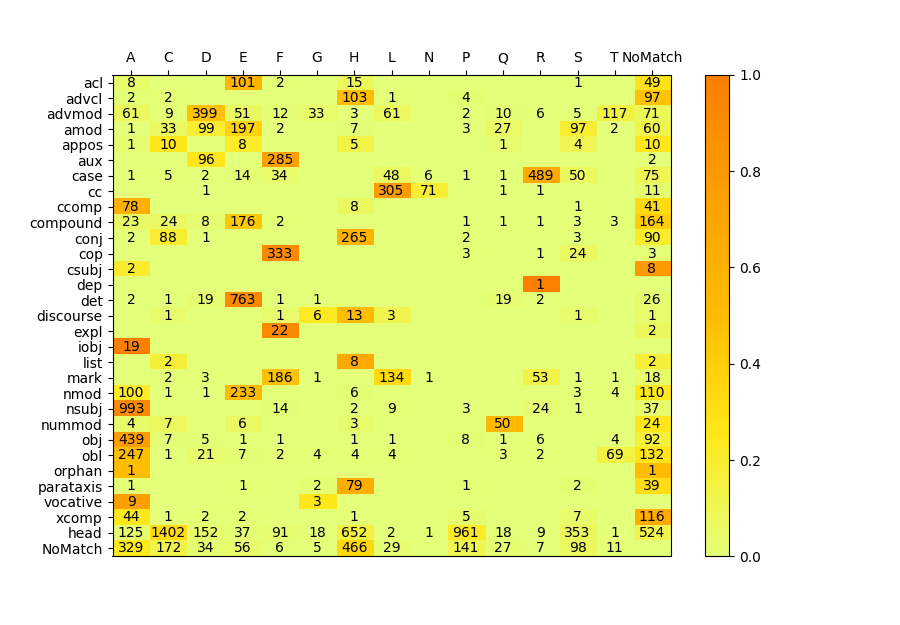
\includegraphics[width=1.15\textwidth]{confusion_matrix.png}
\end{frame}

\begin{frame}
\frametitle{Summary}
\centering
\begin{tabular}{cc}
\bf UCCA & \bf UD \\\\
Scene/non-Scene & POS-based distinction \\\\
primary/secondary relations, & core/non-core arguments \\
participants & \\\\
more MWEs & less MWEs \\\\
Participant/Elaborator/ & coordination/subordination/ \\
Parallel Scenes & complementation/parataxis
\end{tabular}

\begin{minipage}{.4\textwidth}
  \scalebox{.8}{
    \begin{tikzpicture}[level distance=9mm, sibling distance=14mm, ->, draw=Indigo,
        every circle node/.append style={fill=Indigo}]
      \tikzstyle{word} = [font=\rmfamily,color=black]
      \node (ROOT) [circle] {}
        child {node (After) [word] {After} edge from parent node[above] {\scriptsize $L$}}
        child {node (graduation) [circle] {}
        {
          child {node [word] {graduation} edge from parent node[left] {\scriptsize $P$}}
        } edge from parent node[right] {\scriptsize $H$} }
        child {node [word] {,} edge from parent node[below] {\scriptsize $U$}}
        child {node (moved) [circle] {}
        {
          child {node (John) [word] {John} edge from parent node[left] {\scriptsize $A$}}
          child {node [word] {moved} edge from parent node[left] {\scriptsize $P$}}
          child {node [circle] {}
          {
            child {node [word] {to} edge from parent node[left] {\scriptsize $R$}}
            child {node [word] {Paris} edge from parent node[right] {\scriptsize $C$}}
          } edge from parent node[above] {\scriptsize $A$} }
        } edge from parent node[right] {\scriptsize $H$} }
        ;
      \draw[dashed,->] (graduation) to node [above] {\scriptsize $A$} (John);
    \end{tikzpicture}
    }
\end{minipage}
\hfill
\begin{minipage}{.5\textwidth}
    \begin{dependency}[text only label, label style={above,font=\tt\scriptsize, color=DarkBlue}, edge style={color=DarkBlue}, font=\scriptsize\rmfamily]
    \begin{deptext}[column sep=.1em,ampersand replacement=\^]
    After \^ graduation \^ , \^ John \^ moved \^ to \^ Paris \\
    \end{deptext}
        \depedge[edge unit distance=1ex]{2}{1}{case}
        \depedge[edge unit distance=1ex]{4}{3}{punct}
        \depedge[edge unit distance=1ex]{5}{4}{nsubj}
        \depedge[edge unit distance=1ex, edge end x offset=-2pt]{2}{5}{obl}
        \depedge[edge unit distance=1ex]{7}{6}{case}
        \deproot[edge unit distance=1.5ex]{5}{root}
        \depedge[edge unit distance=1.5ex]{5}{7}{obl}
    \end{dependency}
\end{minipage}
\end{frame}

\end{document}
